\noindent
\begin{minipage}[t]{132pt}
    \raggedright
    {\fontsize{20}{24}\selectfont\textbf{\textsf{\color{stewartpurple}Problems Plus}}}\par
    \vspace{56pt}

    \centering
    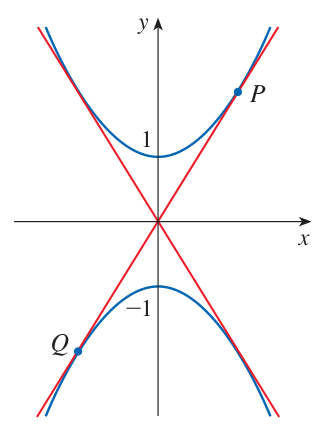
\includegraphics[width=\linewidth]{images/p0309_fig1.png}\par\vspace{4pt}
    {\small\textbf{\textsf{HÌNH 1}}}\par
    \vspace{84pt}

    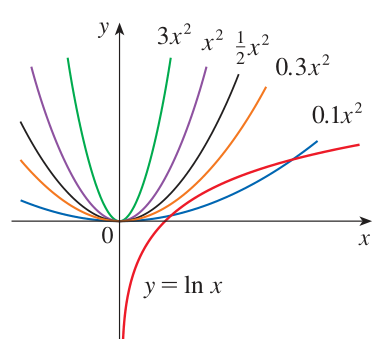
\includegraphics[width=\linewidth]{images/p0309_fig2.png}\par\vspace{4pt}
    {\small\textbf{\textsf{HÌNH 2}}}\par
    \vspace{18pt}

    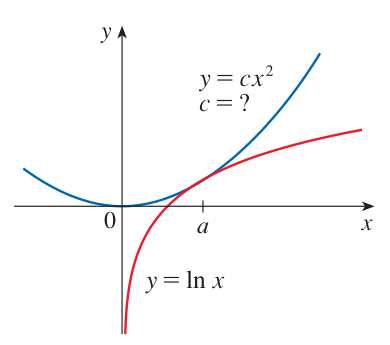
\includegraphics[width=\linewidth]{images/p0309_fig3.png}\par\vspace{4pt}
    {\small\textbf{\textsf{HÌNH 3}}}\par
    \vspace{22pt}

    \raggedright
    {\Large\textbf{\textsf{274}}}\par
\end{minipage}%
\hfill
\begin{minipage}[t]{380pt}
    \vspace*{18pt}
    \setlength{\parindent}{14pt}
    \setlength{\abovedisplayskip}{6pt}
    \setlength{\belowdisplayskip}{6pt}
    \setlength{\abovedisplayshortskip}{3pt}
    \setlength{\belowdisplayshortskip}{3pt}

    \noindent Hãy cố gắng tự mình giải các ví dụ sau đây trước khi đọc lời giải.

    \vspace{10pt}
    \noindent\textbf{\textsf{\color{stewartcyan}VÍ DỤ 1}}\quad Có bao nhiêu đường thẳng đồng thời tiếp xúc với cả hai parabol $y = -1 - x^2$ và $y = 1 + x^2$? Hãy tìm tọa độ của các tiếp điểm mà tại đó các tiếp tuyến này tiếp xúc với các parabol.

    \vspace{6pt}
    \noindent\textbf{\textsf{\color{stewartcyan}LỜI GIẢI}}\quad Để hiểu rõ bản chất của bài toán này, việc phác thảo một hình minh họa là điều cốt yếu. Vì vậy, ta vẽ phác các parabol $y = 1 + x^2$ (là parabol tiêu chuẩn $y = x^2$ được tịnh tiến lên trên 1 đơn vị) và $y = -1 - x^2$ (thu được bằng cách lấy đối xứng parabol thứ nhất qua trục hoành $x$). Nếu thử vẽ một đường thẳng tiếp xúc với cả hai parabol, ta sẽ nhanh chóng nhận ra rằng chỉ có hai khả năng xảy ra, như được minh họa trong Hình 1.

    Gọi $P$ là tiếp điểm mà tại đó một trong các tiếp tuyến này tiếp xúc với parabol phía trên và gọi $a$ là hoành độ của nó. (Việc lựa chọn ký hiệu cho ẩn số là rất quan trọng. Dĩ nhiên chúng ta có thể dùng $b$, $c$, $x_0$ hoặc $x_1$ thay vì $a$. Tuy nhiên, không nên dùng $x$ thay cho $a$ bởi vì ký hiệu $x$ đó có thể gây nhầm lẫn với biến $x$ trong phương trình của parabol.) Khi đó, do điểm $P$ nằm trên parabol $y = 1 + x^2$, tung độ của nó phải bằng $1 + a^2$. Do tính đối xứng thể hiện trong Hình 1, tọa độ của điểm $Q$ nơi tiếp tuyến tiếp xúc với parabol phía dưới phải là $(-a, -(1 + a^2))$.

    Để sử dụng giả thiết đường thẳng là tiếp tuyến, ta cho hệ số góc của đường thẳng $PQ$ bằng hệ số góc của tiếp tuyến tại $P$. Ta có
    \[
    m_{PQ} = \frac{1 + a^2 - (-1 - a^2)}{a - (-a)} = \frac{1 + a^2}{a}
    \]
    \noindent Nếu $f(x) = 1 + x^2$, thì hệ số góc của tiếp tuyến tại $P$ là $f'(a) = 2a$. Do đó, điều kiện mà ta cần sử dụng là
    \[
    \frac{1 + a^2}{a} = 2a
    \]
    \noindent Giải phương trình này, ta thu được $1 + a^2 = 2a^2$, suy ra $a^2 = 1$ và $a = \pm 1$. Do đó, các tiếp điểm là $(1, 2)$ và $(-1, -2)$. Theo tính chất đối xứng, hai tiếp điểm còn lại là $(-1, 2)$ và $(1, -2)$.\hfill\textcolor{stewartcyan}{\rule{1.1ex}{1.1ex}}

    \vspace{10pt}
    \noindent\textbf{\textsf{\color{stewartcyan}VÍ DỤ 2}}\quad Với những giá trị nào của $c$ thì phương trình $\ln x = cx^2$ có đúng một nghiệm?

    \vspace{6pt}
    \noindent\textbf{\textsf{\color{stewartcyan}LỜI GIẢI}}\quad Một trong những nguyên tắc quan trọng nhất trong việc giải toán là vẽ hình minh họa, ngay cả khi đề bài không trực tiếp đề cập đến một tình huống hình học. Vấn đề hiện tại của chúng ta có thể được phát biểu lại dưới góc độ hình học như sau: với các giá trị nào của $c$ thì đường cong $y = \ln x$ cắt đường cong $y = cx^2$ tại đúng một điểm duy nhất?

    Hãy bắt đầu bằng cách vẽ đồ thị hàm số $y = \ln x$ và $y = cx^2$ ứng với các giá trị khác nhau của $c$. Ta biết rằng, với $c \neq 0$, đồ thị $y = cx^2$ là một parabol có bề lõm quay lên trên nếu $c > 0$ và quay xuống dưới nếu $c < 0$. Hình 2 biểu diễn các parabol $y = cx^2$ ứng với một vài giá trị dương của $c$. Phần lớn các parabol này hoàn toàn không cắt $y = \ln x$ và có một parabol cắt tại hai điểm. Ta có cảm nhận rằng phải tồn tại một giá trị nào đó của $c$ (nằm trong khoảng giữa $0{,}1$ và $0{,}3$) sao cho hai đường cong cắt nhau tại đúng một điểm, như được thể hiện trong Hình 3.

    Để tìm giá trị cụ thể đó của $c$, ta gọi $a$ là hoành độ của giao điểm duy nhất nói trên. Nói cách khác, $\ln a = ca^2$, nghĩa là $a$ là nghiệm duy nhất của phương trình đã cho. Từ Hình 3, ta nhận thấy rằng hai đường cong vừa vặn tiếp xúc nhau, vì vậy chúng có chung một tiếp tuyến tại điểm có hoành độ $x = a$. Điều này đồng nghĩa với việc hai đường cong $y = \ln x$ và $y = cx^2$ có cùng hệ số góc khi $x = a$. Do đó
    \[
    \frac{1}{a} = 2ca
    \]
\end{minipage}
